\chapter{Organisation et gestion des données}
%\stepcounter{module}

{\AlegreyaSansLight \large
\begin{center}
\textbf{Crédit :} 11 heures\\
\textit{4 heures hebdomadaires}
\end{center}
}

\minitoc

\section{Introduction}

\subsection{Présentation du module}
Ce module vise à rendre l'apprenant capable de traiter de façon réussie, des situations de vie de la famille  "organisation des données et estimation des quantités dans la consommation des biens et services ". Il s'agit pour lui de :
\begin{itemize}
\item Déployer un raisonnement mathématique pour identifier et formaliser des situations de vie qui se rapportent aux proportionnalités.
\item Résoudre des problèmes relatifs à des situations telles que le placement d'argent, la remise au cours d'achat divers, le partage proportionnel.
\end{itemize}
Pour y parvenir, il est nécessaire de consolider et de renforcer les acquis sur les proportionnalités, les pourcentages et l'échelle vue au cycle primaire tout en restant sur les habiletés cognitives que sont la connaissance, la compréhension et l'application.\\
Ce module est par excellence celui qui, à ce niveau d'étude, comporte les situations de vie les plus familières à l'élève.

\subsection{Contribution du module à la finalité et aux buts curriculaires}
Le module permet de développer les compétences transversales suivantes : le sens de la concision, l'esprit critique et l'organisation rationnelle des données. A terme, ces compétences permettent à l'apprenant de s'assumer comme membre responsable d'une famille, en même temps qu'elles lui permettent d'opérer des choix
judicieux et autonomes, dans la production, la consommation des biens et services.

\subsection{Contribution du module au programme d'études et aux domaines de vie}
Ce module est un des maillons essentiels du programme de 6ème et de 5ème. Il est par excellence l'exemple d'intégration des mathématiques dans la vie quotidienne. Les situations de vie et les exemples d'actions auxquelles il renvoie, de même que toutes les autres composantes du module pourront tout aussi bien intervenir en physique, dans les sciences de la vie et de la terre, en géographie, et plus tard en psychologie et en économie, et surtout dans les situations de vie. Il permet à ce niveau de dégager de manière implicite et même transversale l'importance de l'interdisciplinarité dans plus d'un domaine d'apprentissage.\\
La maîtrise de ces deux notions que ce module développe est de nature à doter l'apprenant d'outils essentiels dont il a besoin dans la vie pratique. Sa contribution dans la gestion du budget familiale est indéniable. Son implication dans la détermination des quantités justifie son importance dans la consommation des biens. Une bonne maîtrise des pourcentages situés (utilisés dans une situation de vie) est un atout majeur dans la consommation des informations, et dans l'exploitation, l'analyse et l'interprétation des données à caractère économique ou social.

\section{Matrice}

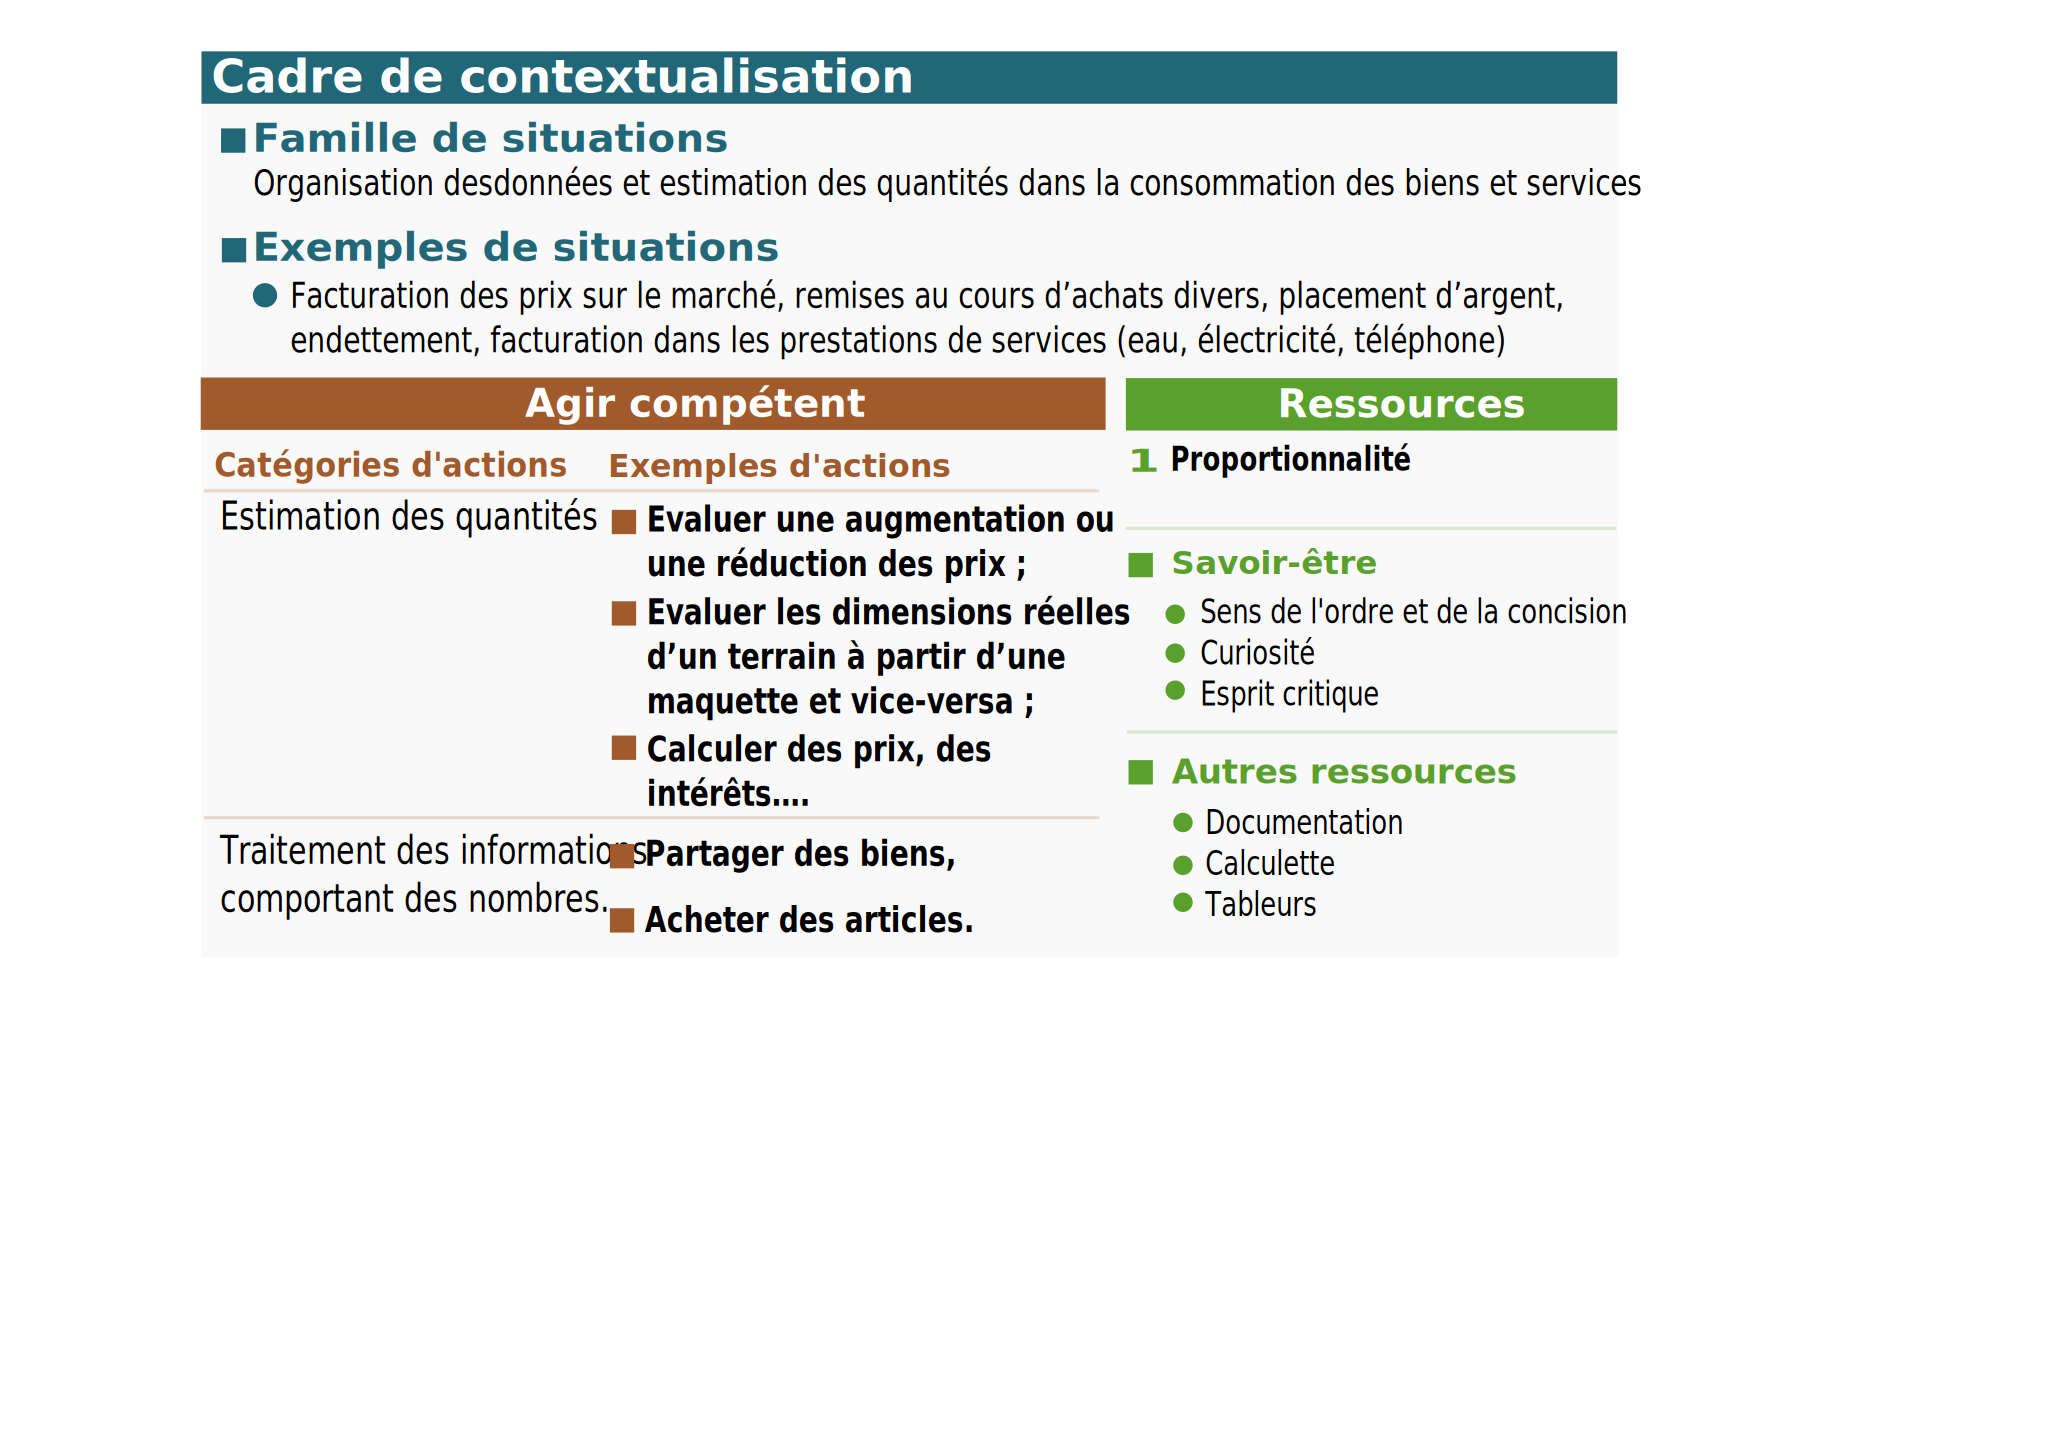
\includegraphics[width=\textwidth]{Module2.pdf} 

\subsection*{}
\addcontentsline{toc}{subsection}{\textbf{Ressource}: proportionnalité}
\ressource{Prop.pdf}

\savoir
\begin{itemize}
\item Tableau de proportionnalité ;
\item Coefficients de proportionnalité ;
\item Suite de nombres proportionnels ;
\item Quatrième proportionnelle ;
\item Pourcentage, échelle ;
\item Propriétés des nombres proportionnels.
\end{itemize}
\savoirfaire
\begin{itemize}
\item Utilisation des coefficients de proportionnalités comme opérateurs ;
\item Utilisation des propriétés des nombres proportionnels pour déterminer des quantités ;
\item Utilisation des pourcentages et des échelles comme opérateurs.
\end{itemize}